O sistema é composto por dois rotores de velocidade variáveis, sendo uma hélice horizontal e outra vertical, acoplado em uma haste com dois graus de liberdade que por sua vez está conectada a uma outra haste com contra-peso.
A planta possui duas variáveis de entrada, que são as tensões de alimentação de cada rotor, fornecidas pela unidade eletrônica, que recebe uma referência de $-2.5$ a $\SI{2.5}{\volt}$ do controlador. Também possui duas variáveis a serem controladas, correspondente aos dois graus de liberdade: ângulo de arfagem e angulo de guinada, sendo sensoreadas, cada uma, por \textit{encoders} incrementais, lidos pela unidade de aquisição de dados e enviados ao controlador \cite{ManualRotor}.

\begin{figure}[H]
    \centering
    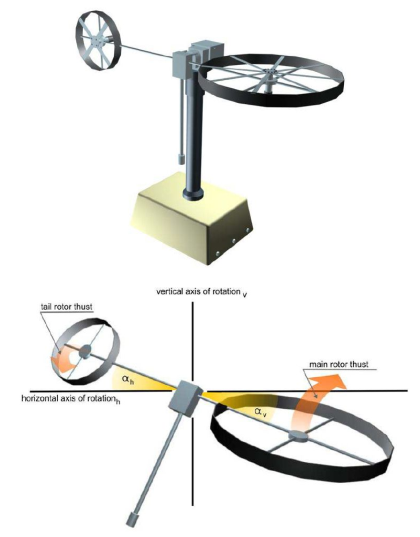
\includegraphics[width=0.30\textwidth]{figures/twin_rotor.PNG}
    \caption{Dispositivo \textit{Twin rotor MIMO System}.}
    \label{fig:TwinRotor}
\end{figure}

No sistema físico está presente a perturbação de fluxos de ar externos e turbulências. Como não-linearidades, tem-se o atraso da aceleração do rotor e de seu empuxo. O torque de arfagem depende de forma não-linear da orientação espacial.

Tem-se como variável controlada o ângulo de arfagem (\textit{pitch angle}), responsável pelo movimento vertical do rotor dianteiro. A tensão aplicada ao rotor é a variável manipulada. O \textit{set-point} ou referência é o ângulo de arfagem desejado, que nessa prática foi expresso em sinais do tipo degrau, senoide e rampa. A variável medida foi o ângulo de arfagem real do rotor (resposta do sistema).

% Para realizar o controlador, optou-se por operar em uma faixa próxima da posição horizontal, a fim de aproximar a planta para um sistema linear.
